\documentclass[a4paper,oneside,12pt]{book}

% #f7efe3

\usepackage[margin=.75in]{geometry}
\usepackage[english]{babel}
\usepackage{microtype}
\usepackage{enumerate}
\usepackage{listings}
\usepackage{hyperref}
\usepackage{graphicx}
\usepackage{float}
\usepackage{blindtext}
\usepackage{color}

\definecolor{lg}{rgb}{.97,.97,.97}
\lstset{
    breaklines=true,
    backgroundcolor=\color{lg},
    captionpos=b,
    basicstyle=\footnotesize\ttfamily,
    frame=shadowbox
}



\title{ECL: Basic Programming \& Machine learning}
\author{Ambu Karthik - 1RV18CS019\\Atreya Bain - 1RV18CS030\\18CS6C5\\Big Data Analytics using Distributed Systems\\R. V. College of Engineering}
\begin{document}
\maketitle{}%
\tableofcontents
\renewcommand{\arraystretch}{1.25}
\pagebreak

\part{ECL Programming}

\chapter{Introduction}

ECL is a declarative language that can be used to work with huge data projects, in the HPCC platform. Its most powerful feature is that you can re-use each query for every subsequent queries. Here's a sample program (It is part of the ECL Playground sample code).

So, breaking it down, there are two types of ECL Code: Definitions, which define what is to be done (eg. loading up a dataset, sorting through a part of a file, and so on) and actions, which are, well, actions; they define what are the actions that are required. Here's a sample program that is from the ECL Playground (most likely the first thing you will see when you load up the playground):

\lstinputlisting[caption={(P0) Comments, Definitions, and Actions},firstline=5]{../source/00-eclStarter.ecl}

The first thing to keep in mind, is that ECL, is \textbf{case-insensitive}. Comments are done in a C/C++ fashion of \lstinline!//! as line-comments and \lstinline!/* */! as block comments. It uses the standard \lstinline!object.property! structure and can be use to nest definitions neatly (Note that it is not an object oriented language).

Execution in ECL, is done by following the trail given by the actions. The execution of an action, requires definitions, which are compiled and executed accordingly. Note that this implies that there \textbf{may not be} an explicit execution order; execution is reordered in a way that helps speed up execution.

Consider the example above, it consists of three definitions, one record, one dataset, and one last definition which is a filter of the previous dataset.
The final line is an action which creates the execution graph. (This is a great segway into the next section.)

\section{Graph Solver}

ECL can actually be considered an optimized graph solver. Digging into ECL Watch, we can obtain this pretty (simple) graph for that previous code sample:
\begin{figure}[h]
    \centering
    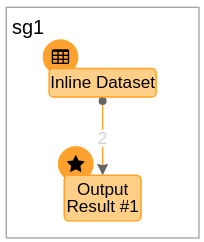
\includegraphics[height=5cm]{../media/simplegraph}
    \caption{Graph for (P0)}
\end{figure}

Each node is some activity, and the (computation) graph is solved in the best possibly way in ECL. The fact that the computation can be very well optimized by mentioning "what" to do, rather than "how" to do, presents a lot of speedups and the ability to parallelize the program as much as possible.

Look at this other example, for which the source code is given:

\lstinputlisting[caption={Source code for the graph below (Don't worry about what's in the code)},firstline=2]{../source/01-graph2.ecl}

\begin{figure}[h]
    \centering
    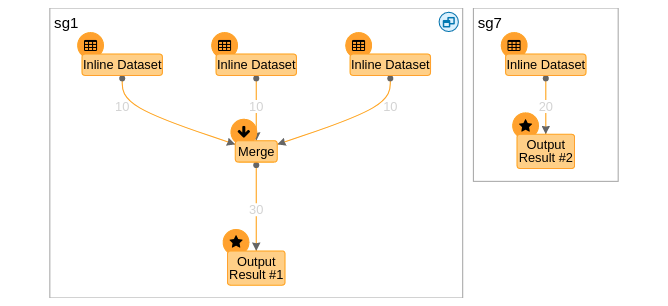
\includegraphics[width=.7\linewidth]{../media/bitlesssimplegraph.png}
    \caption{Bit less simple graph}
\end{figure}

The program above, has two outputs (actions). In this case, two graphs are generated and can be executed accordingly, independently from each other as required. Using this idea, the ECL compiler will compile this ECL code into C++ code that can then be executed on a cluster. This mindset of "graphs" is rather important to the understanding of ECL, as this will help differentiate it from the traditional imperative style of programming.

\section[Chapter information and Datasets]{A rundown of the chapters and datasets used}

The other chapters give examples in ECL, their outputs, and (hopefully) a good understanding of how they work. The last chapter, gives some key methodologies in ECL that is necessary/useful for Machine Learning.

Datasets used have been provided, and can be referred to from the provided repository \url{https://github.com/chrisvrose/bda6-ecl-basics}. Record structures will be given as per the examples, but some corresponding records are also provided for reference.

There are 4 datasets of importance to note:
\begin{enumerate}
    \item heart\_failure.csv - A dataset having 13 attributes of a patient, and whether they have heart disease or not. Refer to the \href{https://www.kaggle.com/ronitf/heart-disease-uci}{kaggle page} for more data. 
    \item house\_prices\_data.csv - A dataset that shows the price of a house, given key attributes about it. Refer to the \href{https://www.kaggle.com/shivachandel/kc-house-data}{user's submission on kaggle} for more data.
    \item Salary\_Data.csv - Years of Experience vs Salary. Its the smallest dataset, and undoubtedly the simplest.
    \item Social\_Network\_Ads.csv - Similar to the earlier dataset, but includes some additional attributes.
    \item vocab.enron.txt - This is a set of words that is used often in machine learning, from the \href{https://archive.ics.uci.edu/ml/datasets/Bag+of+Words}{UCI Machine Learning Repository}
\end{enumerate}

The scope expected in the programs given below is `\~{}eclbasics', but the reader is free to configure them accordingly.

\chapter{Basics}

\section{Data Types}

ECL has a list of basic data types, but more may be derived by the developer.
Some common datatypes are enumerated below. (Use this for quick reference)
\begin{table}[h]
\centering
\begin{tabular}{|c|c|}\hline
Data Type & Description \\\hline\hline
STRING[n] & Packed (or null-terminated) string \\
UTF8 & Unicode character string \\
UNICODE[\_locale][n] &  UTF-16 encoded unicode character string \\
INTEGER[n] & n-byte integer value n can be: 1 - 8 \\
UNSIGNED[n] & n-byte unsigned integer value \\
REAL[n] & n-byte IEEE floating point value \\
DECIMAL\textlangle{}n\textrangle{}[\_y] & Packed decimal value of n total digits \\
BOOLEAN & Boolean value \\
SET OF \textlangle{}type\textrangle{} & A set of values\\
RECORD & Ordered collection of data (Like a tuple)\\
DATASET & Collection of records* \\\hline
\end{tabular}
\caption{Common Data Types}
\end{table}

These data types are used very frequently, and more documentation can be found in the \href{https://hpccsystems.com/training/documentation/learning-ecl}{HPCC Systems Learning ECL} page. Following subsections will start with some programs and how they work.

\subsection[Simple Statistics on Datasets]{(P1) Reading up a dataset and finding some very simple statistics on it}

Scenario: We have a dataset `Salary\_Data.csv', and we want some basic stats on it as sanity checks, before we do some actual work on it. Let's get four things about it:

\begin{enumerate}
    \item Count of rows
    \item Avg years of experience in the dataset
    \item The maximum and the minimum salary that was obtained
    \item The first entry of the dataset.
\end{enumerate}

\lstinputlisting[caption={Program 1 - Sanity checks}]{../source/12-meagre-stats.ecl}

\pagebreak
The output is shown here in XML, but later examples may be shown as table pictures based on the amount of outputs from the program.
This XML output gives a nice description and structure to the output. The result is shown as a set of datasets, which have rows, where values are shown as labelled items.

Some important things to note here, is that ECL arrays, are one-indexed and not zero indexed, like most popular languages. 
Additionally, the `+' operator can perform set operations as well, which we can talk about more later on.
\lstinputlisting[caption={Output 1 - Sanity checks},language=xml]{../output/12/output.xml}



\subsection{Datasets and Records}

\subsubsection[Common data operations]{(P2)Loading up a dataset and working with it}

Being able to filter and process data is rather important. This program should illustrate the common operations that can be done in ECL. This, includes horizontal slicing (filtering), vertical slicing (column-based filters).


\lstinputlisting[caption={(P2)Dataset operations}]{../source/26-common.ecl}


Result 2 and 'projections' will look similar, and that countofYoung is zero. Its an interesting thought, as both can be used for our goal here, but the latter method using projections allow us to refer it later by assigning it to a definition (You can assign an action to a definition, but that is not the same as this). It should also be noted that the \lstinline{TABLE} function can provide a functionality similar to this too, and its functionality is shown later.

Here's the rest of the outputs:

\begin{figure}[h]
    \centering
    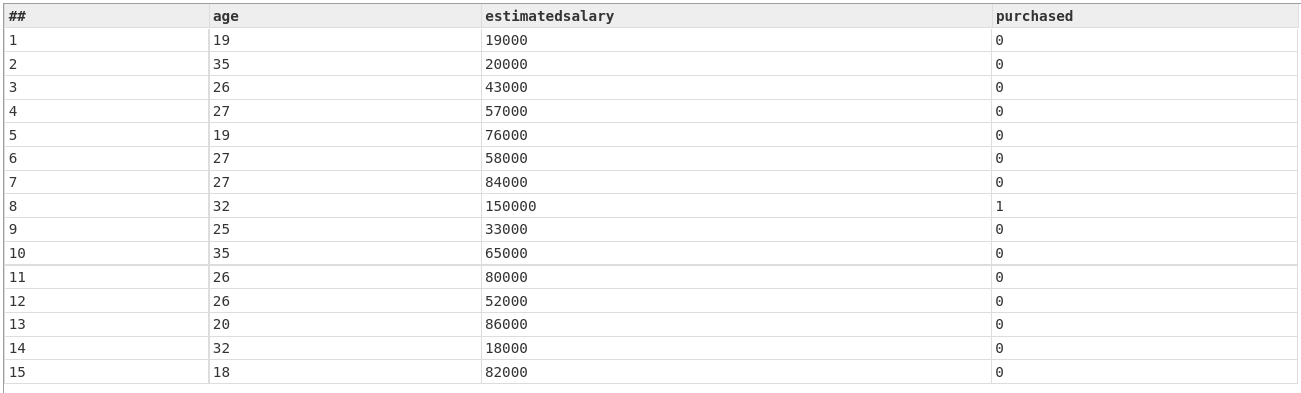
\includegraphics[width=\linewidth]{../output/26/1.png}
    \caption{Result 1 - Output of a segment}
\end{figure}


\begin{figure}[h]
    \centering
    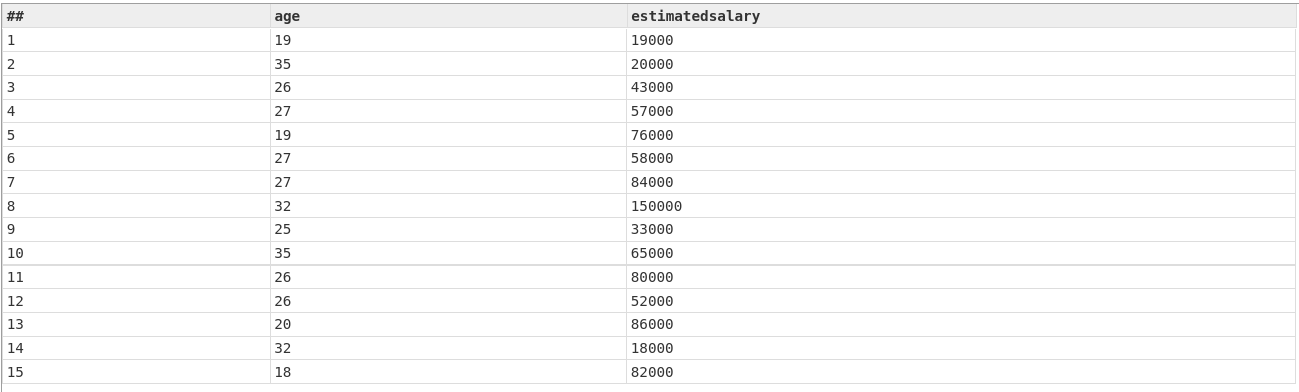
\includegraphics[width=\linewidth]{../output/26/2.png}
    \caption{Result 2 - Output, filtering columns (Only age and salary here)}
\end{figure}

\begin{figure}[h]
    \centering
    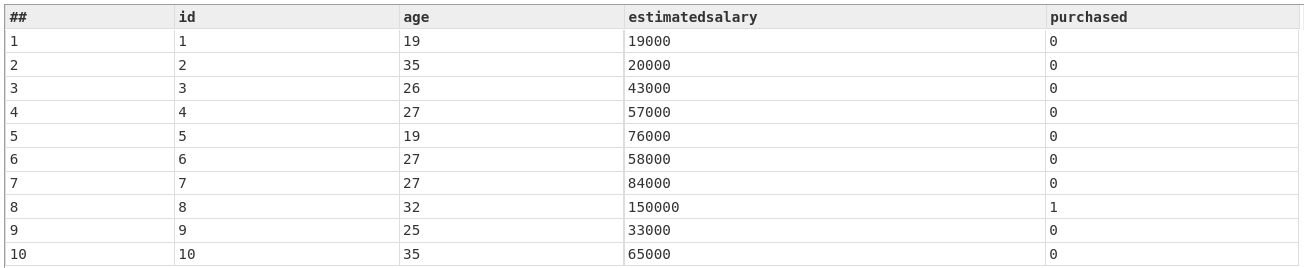
\includegraphics[width=\linewidth]{../output/26/6withid.png}
    \caption{Result 6 - Adding ids with transforms}
\end{figure}


\subsubsection[Filtering \textit{n}\textsuperscript{th} record]{(P3)Filtering by nth record}

Filtering by the nth record is not as unusual as it might look. In ECL, datasets, statements may not may not be order-sensitive, and can be configured as such. This means that the order of the dataset, cannot be ignored, and can be used (Unlike 1NF normalized databases where record positions should never matter).
For a case of \lstinline!n=2!, this problem devolves into picking out every 2nd number, ie. even numbered item.

Let's try the same on \lstinline!Social_Network_Data.csv!, with $n=3$.


\lstinputlisting[caption={(P3) Filtering to n-th record}]{../source/27-nth.ecl}

The output looks rather standard, and there are 134 records output (That's output 2, which is not shown here).

\begin{figure}[h]
    \centering
    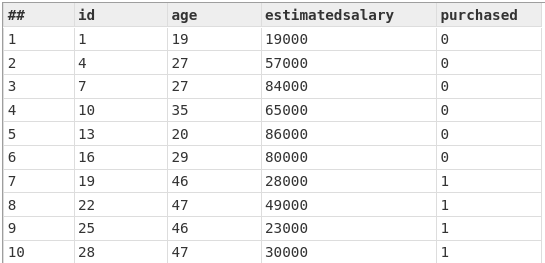
\includegraphics[width=.8\linewidth]{../output/27/1filt_op}
    \caption{Result 1 - Notice that the ids print only the 3rd record}
\end{figure}
\pagebreak
\subsection{Deduplication \& Normalization}

\subsubsection{Deduplication}

For data manipulation, data normalization and dedup play a very large role too. \lstinline{DEDUP} in ECL is a bit special in that you can specify the kind of deduplication wanted. As record order can be made significant; DEDUP can perform dedups locally or over the whole dataset.
The best way to work with \lstinline{DEDUP} is to first sort your data before feeding it to DEDUP. Options for KEEP and BEST can be used for more fine-grained control over how the output dataset will be made.

\lstinputlisting[caption={(P4) Dedup}]{../source/29-dedup.ecl}

The output, is shown here in csv, and looks like:

\lstinputlisting[caption={(P4) Deduplication - Output 1}]{../output/29/WUResult.csv}
\lstinputlisting[caption={(P4) Deduplication - Output 2}]{../output/29/WUResult (1).csv}
\lstinputlisting[caption={(P4) Deduplication - Output 3}]{../output/29/WUResult (2).csv}
\lstinputlisting[caption={(P4) Deduplication - Output 4}]{../output/29/WUResult (3).csv}



\subsection{Normalization}

The \lstinline{NORMALIZE} function `normalizes' child records out of a recordset where the child records are appended to the end of the parent's data records. The purpose is to take a variable-length flat-file recordset, and split out the child information. For those coming from a Spark or JS background, it can be thought of as the \lstinline{.flatMap()} operation. 

Below is one of the two forms of \lstinline{NORMALIZE}.

\lstinputlisting[caption={(P5) Normalize}]{../source/28-normalize.ecl}

The output record, looks like:

\begin{figure}[h]
    \centering
    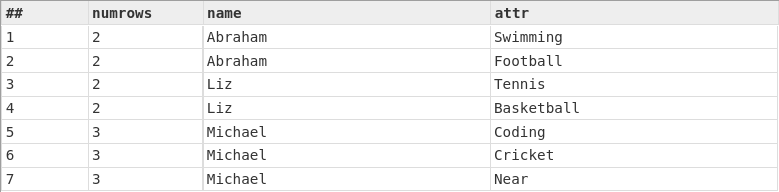
\includegraphics[width=.8\linewidth]{../output/28/1}
    \caption{Result 1 - NORMALIZING}
\end{figure}

\subsection{Iteration \& Recursion}

Functions, unfortunately, may not be called from itself in ECL. This removes the idea of recursion, in ECL.
Instead, we can attempt to use \lstinline{LOOP} to apply tranformations to a dataset.


\subsubsection{(P6) Fibonacci numbers}

\noindent{}Fibonacci sequence generation is a classic iteration/recursion program.
\lstinputlisting[caption={(P6) Fibonacci}]{../source/43-fibonacci.ecl}

The \lstinline!LOOP! function be used to perform an operator multiple times. Note that in this body, the COUNTER keyword is implicitly available for use.

For each successive iteration of \lstinline{LOOP}, the input dataset is the result set of the previous iteration. Let's take a look at the output of the program below.

\begin{figure}[h]
    \centering
    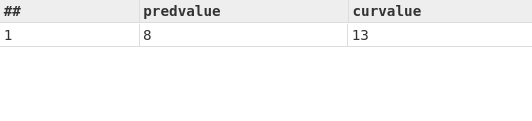
\includegraphics[width=.6\linewidth]{../output/43/op.png}
    \caption{(P6) Output}
\end{figure}

In fact, we can get the final value out of the set by catching the curvalue of the first element of the dataset.

\subsubsection{(P7) Factorial}

A simpler example for how loop works, is the factorial. \lstinline!LOOP! can be used to get the $n!$.
Here's a program and a sample output:

\lstinputlisting[caption={(P7) $10!$}]{../source/44-factorial.ecl}

\begin{figure}[h]
    \centering
    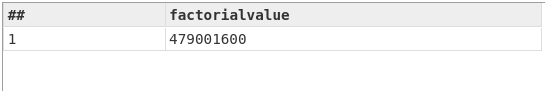
\includegraphics[width=.6\linewidth]{../output/44/1.png}
    \caption{(P7) Output 1}
\end{figure}


\section{ECL and SQL}

Data Analysts may find their needs well expressed in ECL as well. ECL can perform powerful aggregations, filtering, sorting, deduplication and expressive visualizations.

% 3 programs
\subsubsection{Basic SQL comparisons}

ALthough SQL is used mostly in databases, it is a popular choice for data querying and analysis. 
Some comparisons are given below to guide those who have prior knowledge of SQL and also to help show the differences in how SQL and ECL can be used given similar objectives.


\lstinputlisting[caption={(P8) SQL and ECL - Basic querying and aggregtions}]{../source/62-sql1.ecl}

Here's how the output looks like:

\begin{figure}[h]
    \centering
    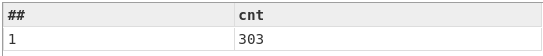
\includegraphics[width=.55\linewidth]{../output/62/1.png}
    \caption{(P8) Output 1 - Number of rows in this dataset}
\end{figure}

\begin{figure}[h]
    \centering
    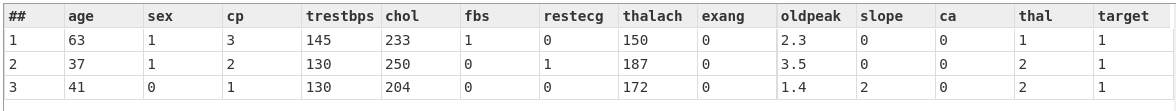
\includegraphics[width=\linewidth]{../output/62/2}
    \caption{(P8) Output 2 - 3 enties of people who have heart disease}
\end{figure}
\begin{figure}[h]
    \centering
    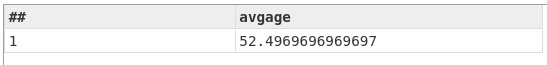
\includegraphics[width=.55\linewidth]{../output/62/3}
    \caption{(P8) Output 3 - The average age of a person who had heart disease}
\end{figure}

\subsection{SQL Queries involving grouping and ordering}

In HPCC Systems, the \lstinline{TABLE} query can also be used to help perform more expressive queries. Grouping and column filtering is possible in one statement here.

\lstinputlisting[caption={(P9) SQL and ECL - Grouping and sorting}]{../source/62-sql1.ecl}

The outputs are as shown:

\begin{figure}[h]
    \centering
    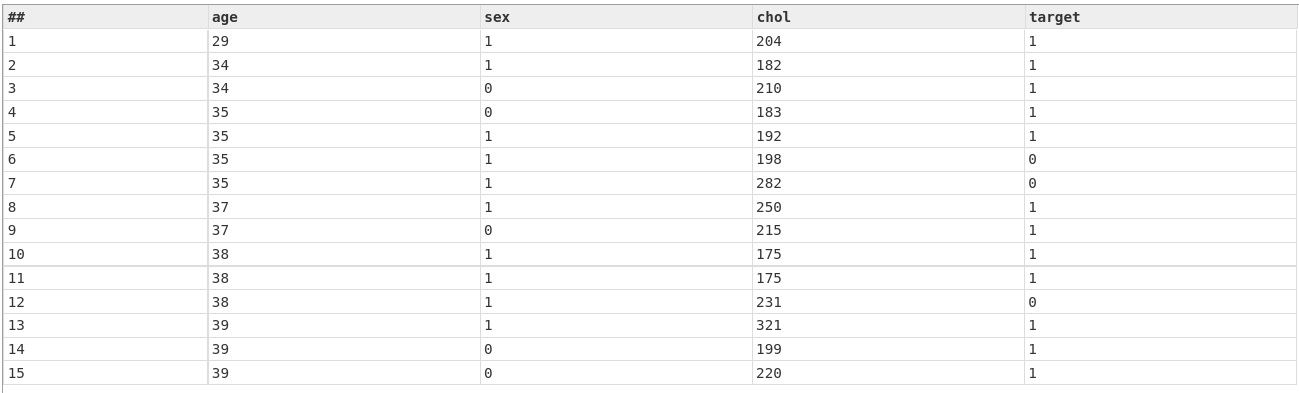
\includegraphics[width=.75\linewidth]{../output/63/1.png}
    \caption{(P9) Output 1 - Information about the youngest few people in this dataset}
\end{figure}

\begin{figure}[h]
    \centering
    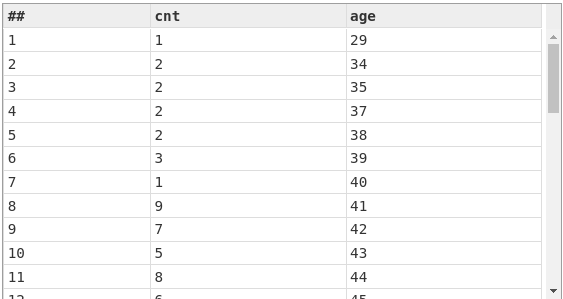
\includegraphics[width=.5\linewidth]{../output/63/2}
    \caption{(P9) Output 2 - A grouped report of age-wise counts of heart disease}
\end{figure}
\begin{figure}[h]
    \centering
    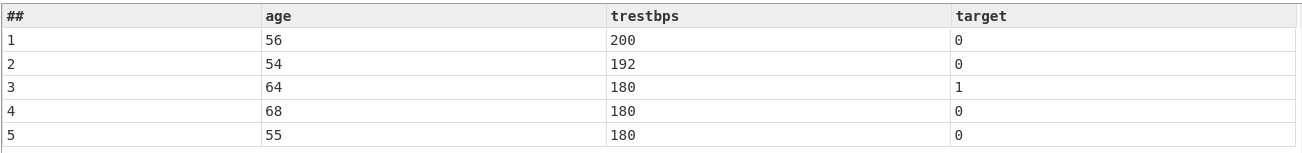
\includegraphics[width=.75\linewidth]{../output/63/3}
    \caption{(P9) Output 3 - The age and the resting heart rate, and whether they had a heart disease, ranked by heart rate}
\end{figure}

\subsubsection{Working with multiple data sources}

SQL queries often support joins to combine data. ECL has the MERGE, and JOIN operators to help with this. Reconsider one of the earlier examples.

MERGE can be used to combine datasets in an efficient manner, although this requires the dataset to be be sorted prior to usage. 
\lstinputlisting[caption={(P10) Merging sorted data},firstline=2]{../source/01-graph2.ecl}

If record order is not constrained, the \lstinline{+} operator may be used. 
However, for constrained based joining of data, JOIN is often used. There are various types of joins, although here only \lstinline{INNER} has been depicted as it is most used. Consider the following example for simple joining.

\lstinputlisting[caption={(P11) Joins}]{../source/64-sql3.ecl}

\begin{figure}[h]
    \centering
    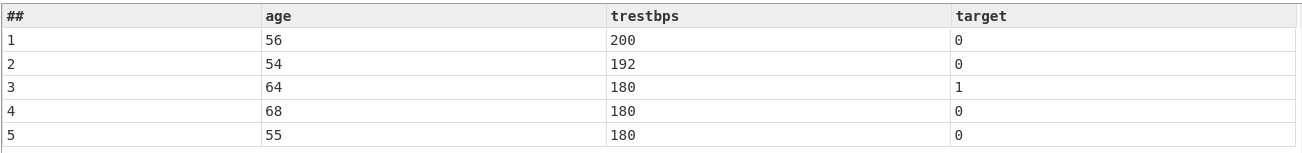
\includegraphics[width=.92\linewidth]{../output/63/3}
    \caption{(P11) Output 1 - Details to bill a person with}
\end{figure}


\chapter{Using Modules}
\section{General module usage}
Modules are a great way to segment your code and split it into separate sections.
Although the \lstinline!.! operator really is reminiscent of OOPs like programming, it is good to remember that ECL does \textit{follow} OOPs.

Consider the following as an example to help explain the various scopes available within a module.
\lstinputlisting[caption={(P12) ./datsrc/modeg.ecl}]{../source/datasrc/modeg.ecl}

\lstinputlisting[caption={(P12) - Using the module}]{../source/75-modules.ecl}

The output, especially showcases the behaviour of default-scoped variables.
\begin{figure}[h]
    \centering
    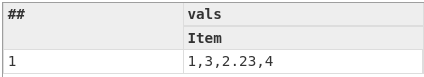
\includegraphics[width=.6\linewidth]{../output/75/1}
    \caption{(P12) Output 1}
\end{figure}

An important point to note is that an ECL program with an export, should not contain actions. This can be understood in the way that export itself is the "output" of the program, ie. the intention of the program is to export these values. This also means that although such programs can be syntax checked, modules cannot be directly executed. However, actions may be tied to definitions and be used in a calling program.


\subsection{Standard library}

The Standard library comes with a lot of very useful functionality for data processing.

\subsubsection[String Handling]{String Handling}

A lot of string handling functions are present as part of the Standard library, and may be used. Note that the \lstinline{TRIM} does not require to be imported from the standard library, even though its primary purpose is string processing.
As a precursor to some other uses, let's consider a case of palindromes, a program that prints out palindromes from a set of words.


\lstinputlisting[caption={(P12) - String handling}]{../source/76-std-stringsimple.ecl}

There are 119 palindromes that come out of our set, and here are a few of them:

\begin{figure}[h]
    \centering
    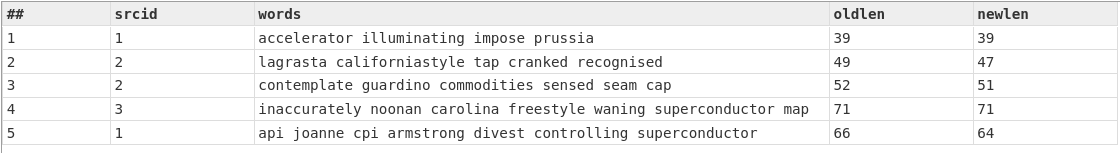
\includegraphics[width=.5\linewidth]{../output/76/1}
    \caption{(P12) Output 1 - Sample of palindromes found}
\end{figure}


The below program recaps some of the earlier concepts on normalize and shows a sample set of data of words, with the objective being to find a set of words which can have some minimal edits to result in the given word.

Right now, the definition \lstinline{word} is hardcoded, but this can be a parameter to a query and this program would extend into a query that would find the minimum edit distance between the words in the dataset.
The final output for 'ap' looks like:

\begin{figure}[h]
    \centering
    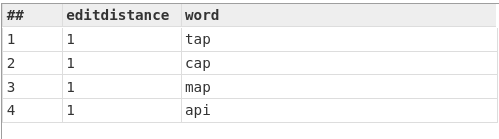
\includegraphics[width=.6\linewidth]{../output/77/5}
    \caption{(P13) Output 5}
\end{figure}

\subsubsection{Date/Time support}

Date Time support is extremely important for any language. The standard library provides a multitude of functions to parse, represent and use date and time values.
Below is a simple example that shows which day of the week today is and what tomorrow is.


\lstinputlisting[caption={(P14) - Date handling}]{../source/78-std-date.ecl}

The output of this program is short, and shows the current date (note that it is pulled in as UTC).

\begin{figure}[h]
    \centering
    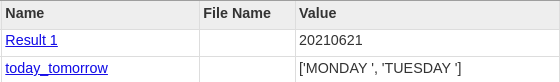
\includegraphics[width=.6\linewidth]{../output/78/1}
    \caption{(P14) Output}
\end{figure}




\subsection{Visualisations}

The \lstinline!Visualizer! is a module that is used for Visualizations, and supports a variety of ways to graph data. There are a variety of visualization formats available but the most common ones are shown here. Some are limited to 2 dimensional data models, whereas some are multidimensional and few are geospatial-based.

Here we plot the marks in a few subjects by the use of the visualizer module.

\lstinputlisting[caption={(P15) - Basic Visualizations}]{../source/79-vis.ecl}


Going to the standard output tab in ECL Watch gives us the data, but we can go to the `Resources tab to view the visualizations'.

(The default header is taken as `Dermatology' for some reason).

\begin{figure}[h]
    \centering
    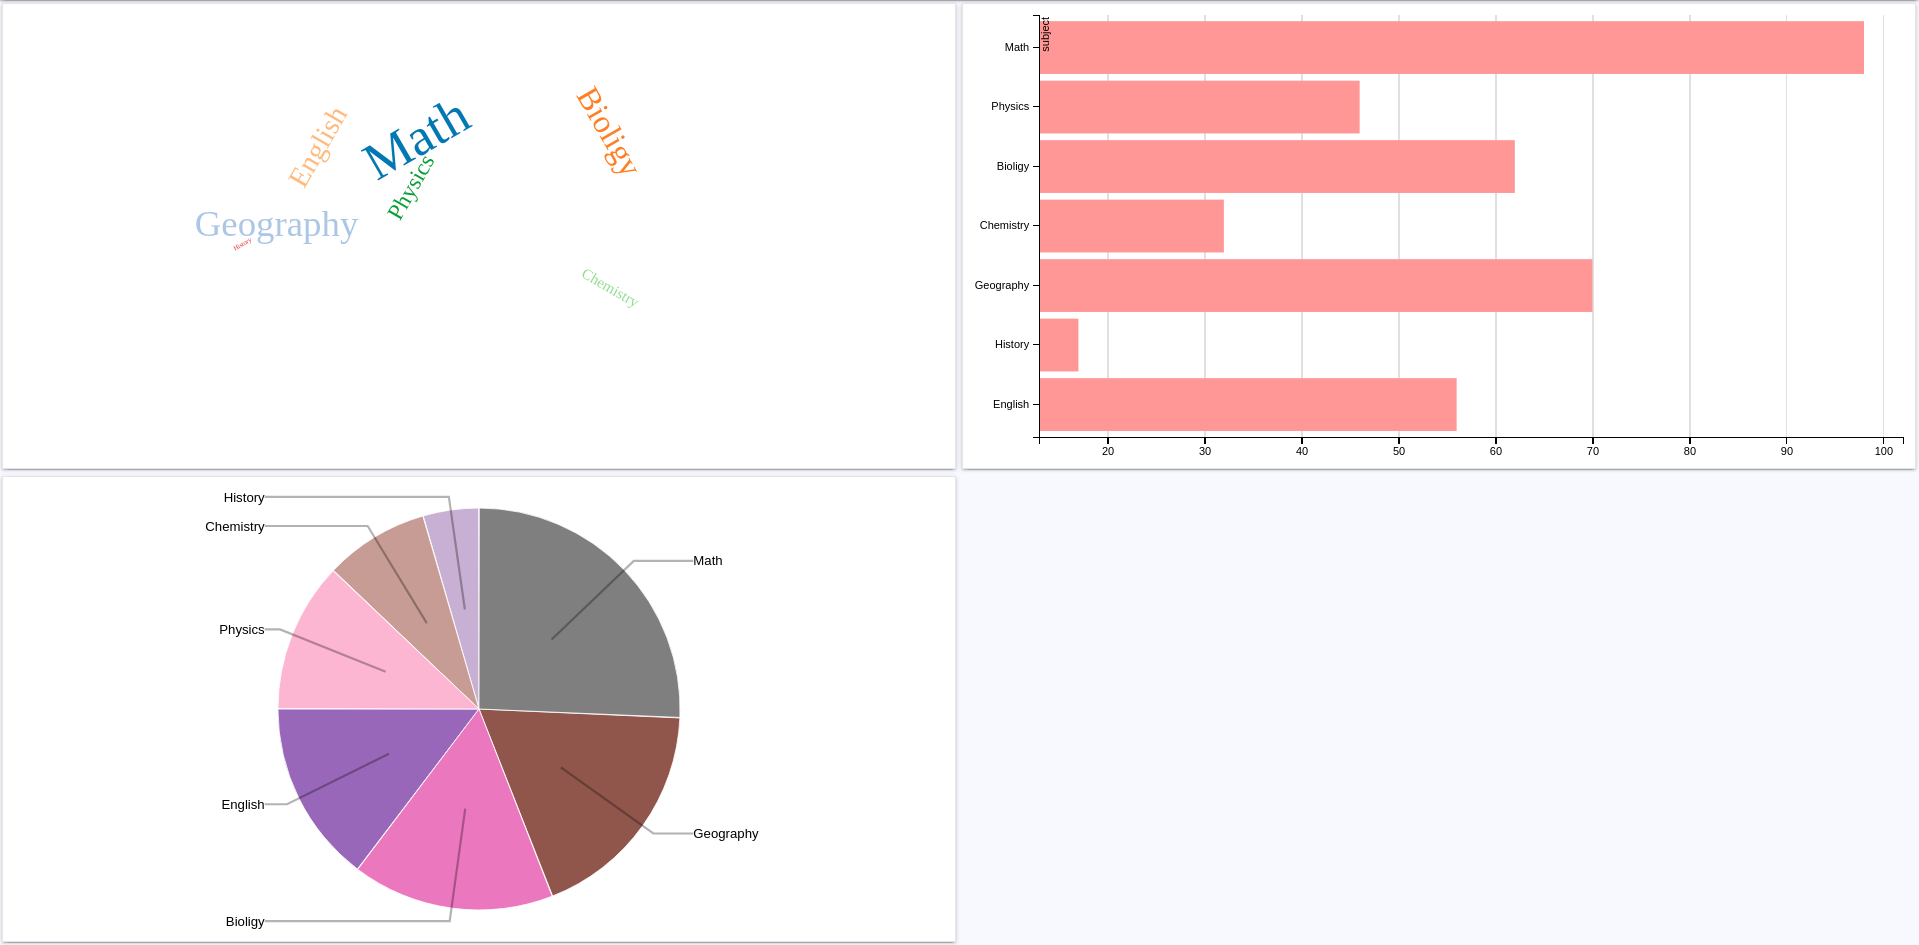
\includegraphics[width=.6\linewidth]{../output/79/1}
    \caption{(P15) Visualization}
\end{figure}




\chapter{Pre-Machine Learning}
\section{Techniques useful for Machine Learning}
\subsection[Dataset Shuffling]{(P16) Dataset Shuffling}

Dataset shuffling is a \textbf{very} important portion of data processing before feeding into machine learning models. This ensures even data distributions and is a good step to perform just before shuffling your dataset (up next).

Now how to shuffle? You can use \lstinline{RANDOM()} to obtain random values in an ECL Program. If this gives an idea, that's great! Adding a field with a value of \lstinline{RANDOM()} and sorting according to it, is a rather effective way to do shuffle a dataset in ECL.

\lstinputlisting[caption={(P16) Shuffle Dataset}]{../source/54-shuffle.ecl}

The output, looks as we would expect. The data has been shuffled. It is important to note that most people don't actually remove the id term, but start using it for an sequential serial id \#. This often goes hand in hand with the fact that HPCC Machine Learning modules expect a first column having a serial \# (Although this can be manually added in with a macro too).

\begin{figure}[h]
    \centering
    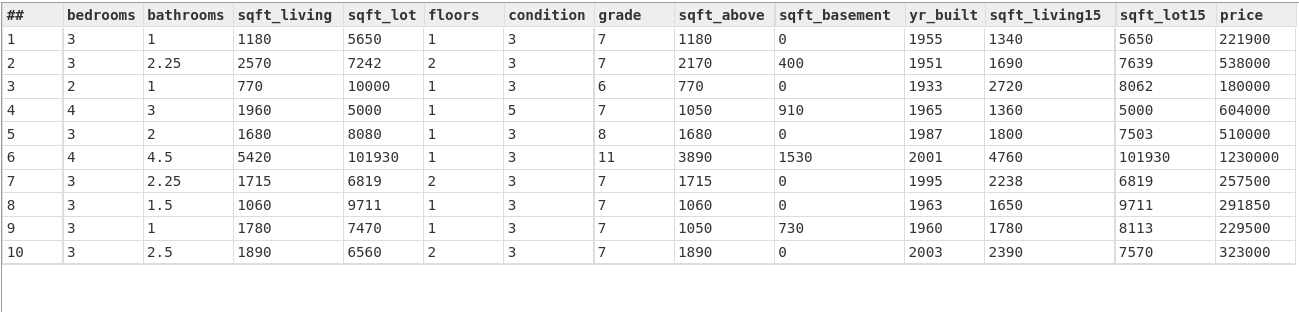
\includegraphics[width=\linewidth]{../output/54/default}
    \caption{Default output}
\end{figure}
\begin{figure}[h]
    \centering
    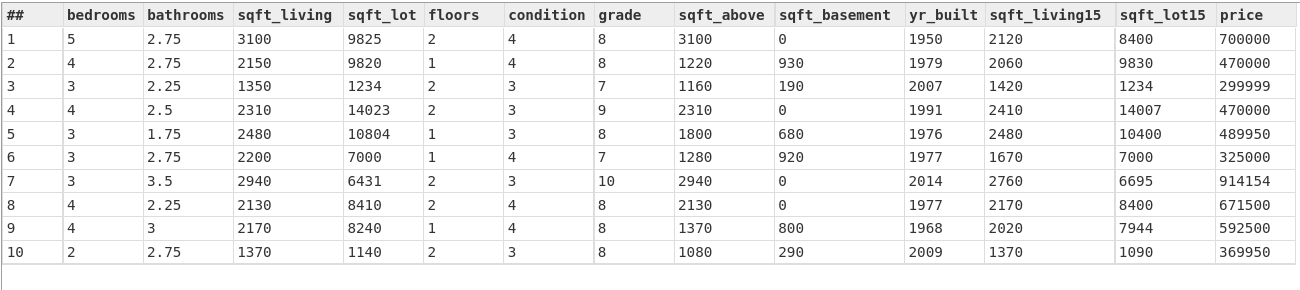
\includegraphics[width=\linewidth]{../output/54/shuffled}
    \caption{Shuffled output}
\end{figure}


\subsection[Dataset Splitting]{(P17) Dataset Splitting}

Dataset splitting is again an important step to working with Machine Learning. Usually, a dataset is split into 2/3 sections, and one set is the training set, and the other is the dev/testing set(s). Once a dataset has been randomized, it can be easily split.

\lstinputlisting[caption={(P17) Split Dataset}]{../source/55-split.ecl}

Here's what the outputs of the program looks:

\begin{figure}[h]
    \centering
    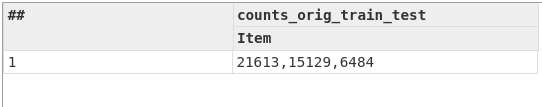
\includegraphics[width=.7\linewidth]{../output/55/counts}
    \caption{Counts $=>$ $6484+15129=21613$}
\end{figure}

\begin{figure}[h]
    \centering
    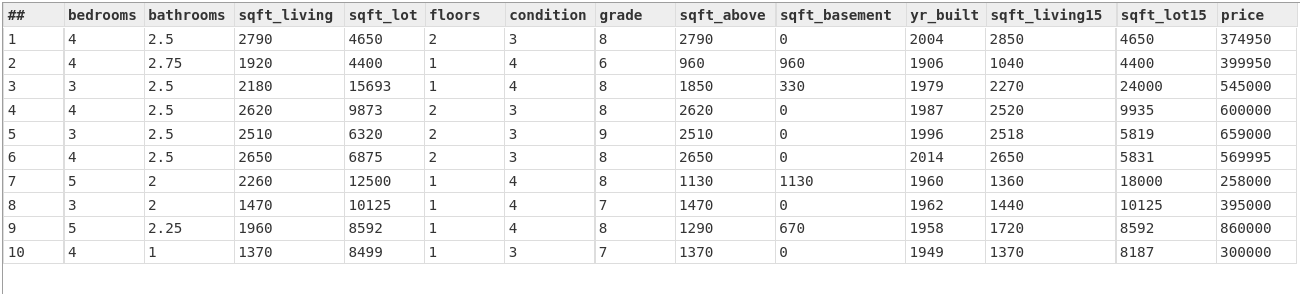
\includegraphics[width=\linewidth]{../output/55/original}
    \caption{Original}
\end{figure}

\begin{figure}[h]
    \centering
    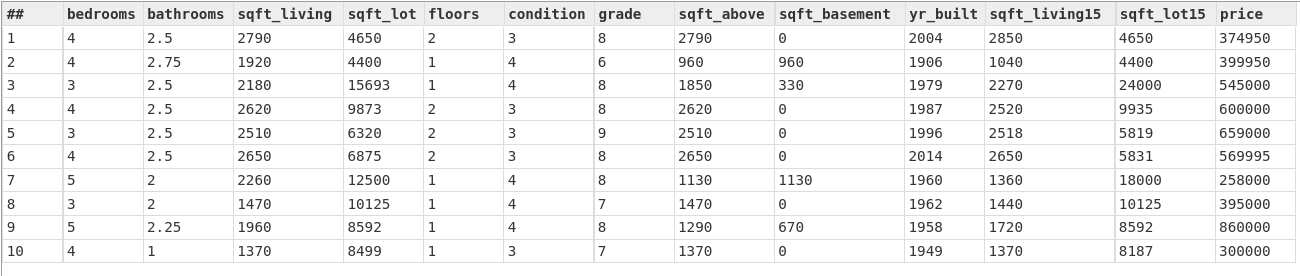
\includegraphics[width=\linewidth]{../output/55/train}
    \caption{Train set excerpt (It looks like the original)}
\end{figure}

\begin{figure}[h]
    \centering
    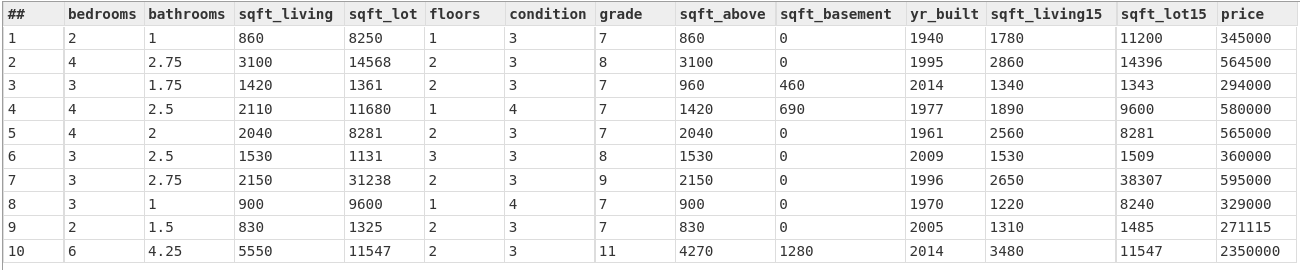
\includegraphics[width=\linewidth]{../output/55/test}
    \caption{Test set excerpt}
\end{figure}

% switch

\part{Prerequisites for Machine Learning in ECL}\label{part:prereqs}

\chapter{Introduction}\label{chap:intro}

Machine learning and Artificial Intelligence are growing at a tremendous rate in the technological world, and most software engineers need knowledge on these fields in order to keep up with the industry.

This brings into light about how training a lot of these models on a large amount of data may take a large amount of time and processing power. To solve these issues, distributed computing was introduced.

Distributed computing is a field of computer science that studies systems whose components are located on different networked computers, which communicate and coordinate their actions by passing messages to one another from any system.

In this document, we shall focus on one such open source distributed system, HPCC Systems. HPCC Systems uses it's own declarative programming language for processing data, which is known as Enterprise Control Language or ECL.

This document assumes that the reader has idea about the following concepts of ECL:
\begin{itemize}
    \item Syntax, Operators
    \item Datasets, Records and Datatypes
    \item Aggregate functions
    \item Sort, Iterate, Rollup, Dedup, Join
    \item Output and Export
    \item Project, Transform, Normalize, Denormalize, Distribute
    \item Functions, Modules and Bundles
\end{itemize}

\section{How to use this document}\label{sec:howtouse}

The best way to use this document would be refer to the parts as it is required by the user after reading through Part \ref{part:prereqs}.

This document is used to help the reader understand how to implement ML algorithms in HPCC systems, but it will be much more useful as a quick reference to using the most important ML methods developed in ECL until \today.

For example, if you ever had to understand how to perform linear regression on your dataset, you could just go to the table of contents to click on the specific part of the linear regression section to make your workflow easier and more convenient.

\section{Supervised vs Unsupervised learning - An overview}\label{sec:supe_vs_unsupe}

Supervised and Unsupervised learning differ in the type of data given to them and in the way they learn. Below is a comic of different kind of robots ranting to each other. Do you think you can figure out the type of learning means from it?

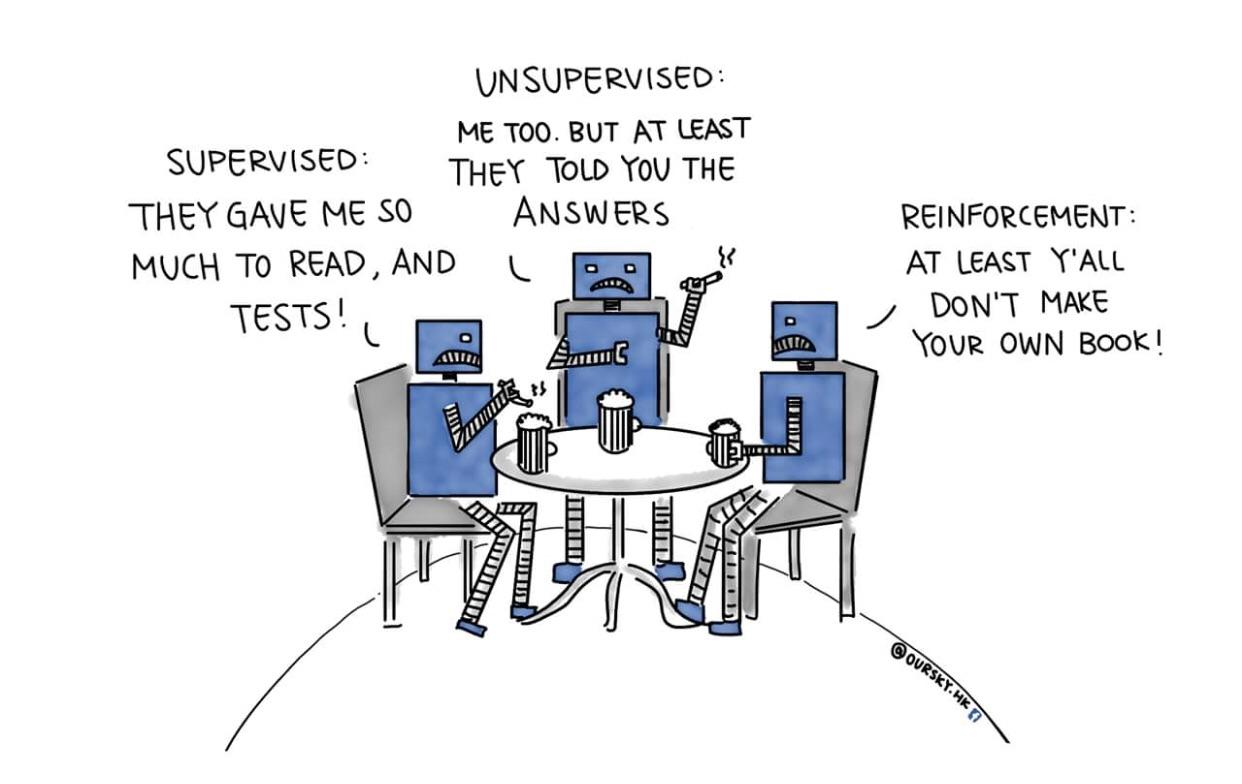
\includegraphics[width=\textwidth]{../media/intro/learningtypes.jpg}

\subsection{Supervised learning}\label{subsec:supe}

When a model trains with data that is well "labelled", and on basis of the given data predicts the output, it is called Supervised learning. It is called so because the training data provided to the model work as the supervisor that teaches the machine to predict correctly. 

Simply explained, the data is like a teacher supervising a student. The teacher must correct the student by showing an example over and over until the student perfectly learns from the examples. The data given to the model acts like the teacher, and is the primary inspiration for the model to predict correctly. 

That being said, it is true that with an incompatible teacher, it might do more worse than good. An teacher specialising in history would be very bad for a student who wants to learn science, and is very interested in it. Just like this, data must be right for the model or it just causes more damage.

Mathematically explained, the aim of supervised learning is to find out the best fitting function $f$ in the equation: \[y=f(x)\] where, $y$ is the predicted output and $x$ is the input variable. 

Supervised learning requires carefully labelled data by a supervisor in order to train the model, and test the accuracy of it to understand and improve the model further.

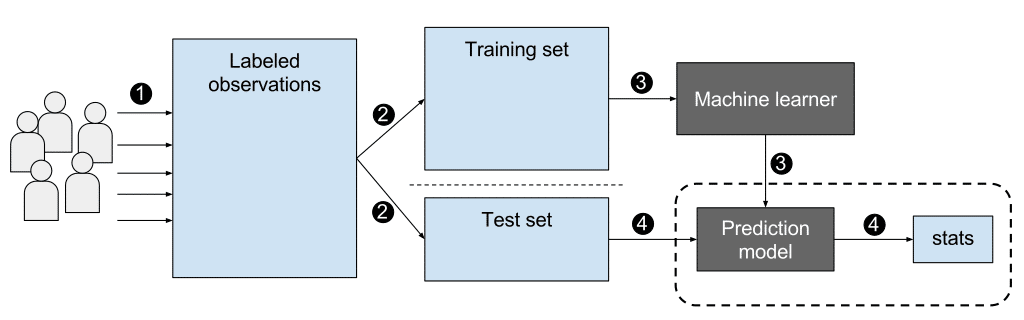
\includegraphics[width=\columnwidth]{../media/intro/Supervised_machine_learning_in_a_nutshell.svg_.png}

The above image explains how supervised learning works in a nutshell. All supervised learning models have the following series of steps that are required to be performed:

\begin{enumerate}
    \item Preparation of labelled data
    \item Pre-processing of data to be compatible with model
    \item Splitting data into train and test sets
    \item Definition of a mathematical model for learning
    \item Train or Fit the model with training set
    \item Test the model with the test set, and calculate accuracy
    \item If accuracy is good enough, use model to predict with real data
\end{enumerate}

That being said, there are many examples of supervised learning models, but the ones available in HPCC Systems developed using ECL or C++ are: 

\begin{itemize}
    \item \nameref{supe:linreg}
    \item \nameref{supe:logreg}
    \item \nameref{supe:svm}
    % \item \nameref{supe:glm}
    \item \nameref{supe:learntrees}
    % \item \nameref{supe:gnn}
\end{itemize}

All the above listed bundles are explained in the following document in Part \ref{part:supe}.

\subsection{Unsupervised learning}\label{subsec:unsupe}

When a model trains with data that is unlabelled, and are allowed to act on the data without supervision, it is called Unsupervised learning. Unlike in supervised learning, the data does not act as a supervisor to the model.

Simply explained, here the data is like homework provided by the teacher to the student. The student must look at the homework, and based on existing knowledge must figure out patterns, and extrapolate answers. Just like this, in unsupervised models, there are no corrections done, but the model must work on the data without supervision in order to learn from the patterns in the data, because the data doesn't have answers provided in it. 

Here as well, it is true that with homework that don't have existing patterns or are beyond the scope of the student will be filled by bizarre answers by the student. Similarly, if a certain dataset is beyond the scope of an unsupervised model, it will provide bizarre results.

Unsupervised learning requires unlabelled data along with a specific model with the perfect parameters to yield the best results. The model fits onto the dataset, and then is tested to check for best results. Then the model is further improved until it works best for the dataset provided.
\\

All unsupervised learning models have the following series of steps that are required to be performed:

\begin{enumerate}
    \item Ponder on the application and the kind of data being used
    \item Choose the model appropriately
    \item Preprocess the data to be compatible with the model
    \item Define the mathematical model that will be used
    \item Split the dataset into train and test sets
    \item Fit the train data to the model
    \item Test the model with the test set, and calculate accuracy
    \item If accuracy is good enough, use model to work with real data
\end{enumerate}

There are many examples of unsupervised learning models, but the ones available in HPCC Systems developed using ECL or C++ are:

\begin{itemize}
    \item \nameref{unsupe:kmeans}
    \item \nameref{unsupe:dbscan}
\end{itemize}

All the above listed bundles are explained in the following document in Part \ref{part:unsupe}

\chapter{The Core and Building Blocks of ML}\label{chap:coreml}

All these Machine Learning algorithms have a lot of mathematics with topics spanning over Linear Algebra, Calculus, Statistics, Probability, Geometry and Decision theory as well. 

Most of the algorithms are a combination of multiple mathematical operations/functions used together in all steps of performing machine learning. 

The most commonly used ones need to be written in the most optimised manner for the ease of the data scientist/programmer so they can focus on the ML algorithm or task at hand instead of needing to gain a deep understanding of how each mathematical operation and function work to implement them, and then putting them together for the ML algorithm.

This is where the bundles \nameref{sec:mlcore} and \nameref{sec:pbblas} come in. These bundles contain the most essential mathematical functions that are used in the ML algorithms to give a simple interface for the user of HPCC to work with the models and datasets conveniently.

\section{ML Core}\label{sec:mlcore}

ML Core simply abbreviates to "Machine Learning Core", and it defines the required functions that are needed for Data Manipulation, Analysis and Model evaluation. This section will be covering about the installation, usage and the most commonly used functions in ML Core.

\subsection{Installation}

To install this bundle, the user needs to run the following command:

\begin{lstlisting}[language=bash]
$ ecl bundle install https://github.com/hpcc-systems/ML_Core
\end{lstlisting}

This will install the latest stable version of ML Core from the official repository.

\subsection{Usage}

Although the bundle is installed, the user still needs to IMPORT the bundle into their ECL code. The required functions need to be imported and used accordingly as per the use case.

An example given below shows the usage of an important macro \textbf{\nameref{mlcore:tofield}}:

\begin{lstlisting}
IMPORT ML_Core;

exampleRec := RECORD
    INTEGER id;
    REAL value;
END;

exampleDs := DATASET('~example::example.csv', 
                    exampleRec, CSV(HEADING(1),
                    SEPARATOR(','),
                    TERMINATOR(['\n','\r\n','\n\r'])));

ML_Core.ToField(exampleDs, exampleNF);
OUTPUT(exampleNF);
\end{lstlisting}

There's a deep documentation file of ML Core that can be accessed on the HPCC website on the following link: \url{https://cdn.hpccsystems.com/pdf/ml/ML\_Core.pdf}. This documentation has the official declaration of parameters, return types and bundle structure. This can be used for reference and importing from ML Core properly. This document goes with a more example-oriented approach to understand the bundles described.

\subsection{Commonly used functions}

\subsubsection{ToField}\label{mlcore:tofield}

\textit{Converts a record-oriented dataset to a cell-oriented NumericField dataset for use with Machine Learning mechanisms}

\paragraph{Explanation}

By \textbf{Record-oriented dataset}, it really refers to most ECL datasets that really on a specific record. For example, I can have id, name, email id, date of birth be defined as a record like this:

\begin{lstlisting}
exampleRec := RECORD
    INTEGER id;
    STRING name;
    STRING emailid;
    DATE dob;
END;
\end{lstlisting}

The problem with this kind of structure is that specific cells of data cannot be dealt with easily. I would have to ingest record-by-record, which may not be correct for ML operations as a few attributes will not be needed at all.

To solve this issue, certain uniform formats for all ML algorithms in ECL are used by ML Core which are NumericField and DiscreteField. These are defined in Types.ecl module in ML Core bundle. These are \textbf{Cell-oriented} which means that data can be handled as independent cells having values with a certain position defined based on column and rowID. More can be read in the documentation that was talked about above.

\paragraph{Example}

Let's look at an example using ML Core to understand better on how to use it.

\begin{lstlisting}
IMPORT ML_Core;

exampleRec := RECORD
    INTEGER id;
    STRING name;
    STRING emailid;
    REAL marks;
    INTEGER studytime;
END;

exampleDs := DATASET('~example::example.csv', 
                    exampleRec, CSV(HEADING(1),
                    SEPARATOR(','),
                    TERMINATOR(['\n','\r\n','\n\r'])));

ML_Core.ToField(exampleDs, exampleNF);
OUTPUT(exampleNF);
\end{lstlisting}

An example record is defined above which defines the shape of each record in the dataset. A dataset is created from a sprayed CSV file in a specific format. This dataset is converted to a Numeric Field for ML applications.

A question might arise: exampleNF is not even defined. How are we giving it as an argument?

This is where the term "Macros" in ECL come into application. A macro does not return anything but new attributes are created in-line for use in subsequent definitions. ToField is a Macro that defines exampleNF for use in further definitions and it does not need to be defined explicitly.

The above code can be run with any CSV file and record to observe the Numeric Field format and get a better understanding of how it works.

\textbf{Note}: All the arguments after exampleRec in the DATASET function in the above example are specific to a CSV file.

\subsubsection{FromField}\label{mlcore:fromfield}

\textit{Macro to convert a NumericField formatted, cell-based dataset to a Record formatted dataset}

\paragraph{Explanation}

This macro does the exact opposite of ToField. It takes a Numeric Field and converts it into a specific record-oriented dataset. 

It really comes to use to convert the output of regressional models into record-oriented dataset to analyse and read better. 

\paragraph{Example}

Let's look at an example of FromField being used

\begin{lstlisting}
IMPORT ML_Core;

exampleRec := RECORD
    INTEGER id;
    STRING name;
    STRING emailid;
    REAL marks;
    INTEGER studytime;
END;

exampleDs := DATASET('~example::example.csv', 
                    exampleRec, CSV(HEADING(1),
                    SEPARATOR(','),
                    TERMINATOR(['\n','\r\n','\n\r'])));

ML_Core.ToField(exampleDs, exampleNF);
OUTPUT(exampleNF);

ML_Core.FromField(exampleNF, exampleRec, exampleDsOut);
OUTPUT(exampleDsOut);
\end{lstlisting}

The above example shows how to convert any Numeric Field into a record-oriented dataset given a record. FromField is a macro so exampleDsOut can be used in subsequent lines as it's defined in-line.

\subsubsection{AppendID}\label{mlcore:appendid}

\textit{Macro takes any structured dataset, and appends a unique 1-based record ID column to it. Values will not be sequential and values will not be dense because of data skew. Gaps will appear when data ends on each node. If dense and sequential values are required, use \nameref{mlcore:appendseqid}.}

\paragraph{Example}

Here's an example of AppendID to show it can be used in ECL

\begin{lstlisting}
IMPORT ML_Core;

exampleRec := RECORD
    STRING name;
    STRING emailid;
    REAL marks;
    INTEGER studytime;
END;

exampleDs := DATASET('~example::example.csv', 
                    exampleRec, CSV(HEADING(1),
                    SEPARATOR(','),
                    TERMINATOR(['\n','\r\n','\n\r'])));

ML_Core.AppendID(exampleDs, id, exampleDsID);
OUTPUT(ML_Core);
\end{lstlisting}

NumericField will had IDs by itself when not mentioned, but it's a good practice to append IDs to the dataset by using the Append ID macros. The second argument mentions what the attribute name of the appended ID will be.

\subsubsection{AppendSeqID}\label{mlcore:appendseqid}

\textit{Macro takes any structured dataset, and appends a unique 1-based record ID column to it. Values will be in data sequence. Note: implemented as a count project, each node processes the data in series instead of parallel. For better cluster performance, use \nameref{mlcore:appendid} as long as dense, sequential ids are not needed.}

\paragraph{Example}

Here's an example of AppendSeqID to show how it can be used in ECL

\begin{lstlisting}
IMPORT ML_Core;

exampleRec := RECORD
    STRING name;
    STRING emailid;
    REAL marks;
    INTEGER studytime;
END;

exampleDs := DATASET('~example::example.csv', 
                    exampleRec, CSV(HEADING(1),
                    SEPARATOR(','),
                    TERMINATOR(['\n','\r\n','\n\r'])));

ML_Core.AppendSeqID(exampleDs, id, exampleDsID);
OUTPUT(ML_Core);
\end{lstlisting}

NumericField will had IDs by itself when not mentioned, but it's a good practice to append IDs to the dataset by using the Append ID macros. The second argument mentions what the attribute name of the appended ID will be.

\subsubsection{Discretize}\label{mlcore:discretize}

\textit{This module is used to turn a dataset of NumericFields into a dataset of DiscreteFields. This is not quite as trivial as it seems as there are a number of different ways to make the underlying data discrete; and even within one method there may be different parameters. Further - it is quite probable that different methods are going to be desired for each field.}

\paragraph{Functions}

\begin{enumerate}
    \item \textbf{ByRounding}: Round the values passed in to create a discrete element Scale is applied (by multiplication) first and can be used to bring the data into a desired range.
    \item \textbf{ByBucketing}: Allocates a continuous variable into one of N buckets based upon an equal division of the RANGE of the variable.
    \item \textbf{ByTiling}: Allocate a continuous variable into one of N groups such that each group (tile) contains roughly the same number of entries and that all of the elements of group 2 have a higher value than group 1, etc.
\end{enumerate}

\begin{lstlisting}
IMPORT ML_Core;

exampleRec := RECORD
    INTEGER id;
    STRING name;
    STRING emailid;
    INTEGER age;
    BOOLEAN bookBought;
END;

exampleDs := DATASET('~example::example.csv', 
                    exampleRec, CSV(HEADING(1),
                    SEPARATOR(','),
                    TERMINATOR(['\n','\r\n','\n\r'])));

ML_Core.ToField(exampleDs, exampleNF);
OUTPUT(exampleNF);

// Discretization by Rounding values (1st Method)
rounded := ML_Core.Discretize.ByRounding(exampleNF);
OUTPUT(rounded, NAMED('ByRounding'));

// Discretization by Bucketing (2nd Method)
bucketed := ML_Core.Discretize.ByBucketing(exampleNF);
OUTPUT(bucketed, NAMED('ByBucketing'));

// Discretization by Tiling (3rd Method)
tiled := ML_Core.Discretize.ByTiling(exampleNF);
OUTPUT(tiled, NAMED('ByTiling'));
\end{lstlisting}

Discretization is important to generate DiscreteField dataset for Classification problems as classifiers rely on DiscreteField and NumericField are incompatible. It's use is shown in the program given in Classification Analysis Example and all classification models in the following document.

\subsubsection{Analysis}\label{mlcore:analysis}

\textit{Analysis is a module in ML Core that has functions defined to analyse the trained models of any kinds to check for it's performance on a certain dataset. }

\paragraph{Classification}\label{analysis:classification}

\textit{This sub-module provides functions for analyzing and assessing the effectiveness of an ML Classification model. It can be used with any ML Bundle that supports classification.}

\subparagraph{Functions}

All of these will be implemented in a further example

\begin{enumerate}
    \item \textbf{ClassStats}: Given a set of expected dependent values, assess the number and percentage of records that were of each class.
    \item \textbf{ConfusionMatrix}: Returns the Confusion Matrix, counting the number of cases for each combination of predicted Class and actual Class.
    \item \textbf{Accuracy}: Assess the overall accuracy of the classification predictions
    \item \textbf{AccuracyByClass}: Provides per class accuracy along with relevance statistics like Precision, Recall, False-positive Rate.
\end{enumerate}

\subparagraph{Example}\label{classification:example}

Given below is an ECL code implementing Classification Forests using Learning Trees. This will show how all the ML Core functions shown above are used with any classification model.

\begin{lstlisting}
IMPORT ML_Core;
IMPORT LearningTrees; // We are using Learning Trees here. Shall be covered in a further chapter
IMPORT $ as root; // Importing current folder to get dataset

RFClassDs := root.Datasets.heartDs.Ds; // This is a dataset that is not relevant to us, it's just an example

// Get count of how many records to split to train and test dataset
recordCount := COUNT(RFClassDs);
splitRatio := 0.8;

// Record that is used to shuffle dataset
Shuffler := RECORD(RECORDOF(RFClassDs))
  UNSIGNED4 rnd; // A random number
END;

newDs := PROJECT(RFClassDs, TRANSFORM(Shuffler, SELF.rnd := RANDOM(), SELF := LEFT)); 

shuffledDs := SORT(newDs, rnd); // Shuffle by sorting a list of random numbers

// Train and Test dataset splitting
TrainDs := PROJECT(shuffledDs[1..(recordCount * splitRatio)], RECORDOF(RFClassDs));
TestDs := PROJECT(shuffledDs[(recordCount*splitRatio + 1)..recordCount], RECORDOF(RFClassDs));

OUTPUT(TrainDs, NAMED('TrainDataset'));
OUTPUT(TestDs, NAMED('TestDataset'));

// Appending IDs as the original data does not have it
ML_Core.AppendSeqID(TrainDs, id, newTrain);
ML_Core.AppendSeqID(TestDs, id, newTest);

OUTPUT(newTrain, NAMED('TrainDatasetID'));
OUTPUT(newTest, NAMED('TestDatasetID'));

// Converting data to Numeric Field
ML_Core.ToField(newTrain, TrainNF);
ML_Core.ToField(newTest, TestNF);

OUTPUT(TrainNF, NAMED('TrainNumericField'));
OUTPUT(TestNF, NAMED('TestNumericField'));

// Getting dependent(y) and independent(x) variables separated in both train and test datasets
independent_cols := 13;

X_train := TrainNF(number < independent_cols + 1);
y_train := ML_Core.Discretize.ByRounding(PROJECT(TrainNF(number = independent_cols + 1), TRANSFORM(RECORDOF(LEFT), SELF.number := 1, SELF := LEFT)));

X_test := TestNF(number < independent_cols + 1);
y_test := ML_Core.Discretize.ByRounding(PROJECT(TestNF(number = independent_cols + 1), TRANSFORM(RECORDOF(LEFT), SELF.number := 1, SELF := LEFT)));

OUTPUT(y_test, NAMED('ActualY'));

\\ Check the class stats of testY (1st function)
stats := ML_Core.Analysis.Classification.ClassStats(y_test);
OUTPUT(stats, NAMED('ClassStats'));

\\ Learning Trees Classifier model fitting over train set
classifier := LearningTrees.ClassificationForest().GetModel(X_train, y_train);

\\ Predicting over fitted model with test dataset
predicted := LearningTrees.ClassificationForest().Classify(classifier, X_test);
OUTPUT(predicted, NAMED('PredictedY'));

\\ Generate confusion matrix with predicted and actual values (2nd function)
cm := ML_Core.Analysis.Classification.ConfusionMatrix(predicted, y_test);
OUTPUT(cm, NAMED('ConfusionMatrix'));

\\ Calculate overall classification accuracy of model (3rd function)
accuracy_values := ML_Core.Analysis.CLassification.Accuracy(predicted, y_test);
OUTPUT(accuracy_values, NAMED('AccuracyValues'));

\\ Calculate classification accuracy by class of model (4th function)
accuracy_by_class := ML_Core.Analysis.Classification.Accuracy(predicted, y_test);
OUTPUT(accuracy_by_class, NAMED('AccuracyByClass'));
\end{lstlisting}

The above code sums up all of ML Core functionality in a clean classification problem. It should be similar for most classification models in ECL.

\paragraph{Regression}\label{analysis:regression}

\textit{This sub-module provides functions for analyzing and assessing the effectiveness of an ML Regression model. It can be used with any ML Bundle that supports regression.}

\subparagraph{Functions}

Regression has just one function in Analysis which is:

\textbf{Accuracy}: Assess the overall accuracy of the regression predictions

This will be implemented in the upcoming example

\subparagraph{Example}\label{regression:example}

Given below is an ECL code implementing Regression Forests using Learning Trees. The following code will show how all the functions in ML Core discussed above are used with a regression model.

\begin{lstlisting}
IMPORT ML_Core;
IMPORT LearningTrees; // Using Learning Trees regression as example
IMPORT $ as root; // Importing directory to get dataset

RFRegDs := root.Datasets.houseDs.Ds; // Irrelevant dataset, just as an example

// Counting total number of records to split dataset
recordCount := COUNT(RFRegDs);
splitRatio := 0.8;

// Shuffling dataset using shuffler record and sorting
Shuffler := RECORD(RECORDOF(RFRegDs))
  UNSIGNED4 rnd; // A random number
END;

newDs := PROJECT(RFRegDs, TRANSFORM(Shuffler, SELF.rnd := RANDOM(), SELF := LEFT));

// Sorts dataset over random numbers to shuffle
shuffledDs := SORT(newDs, rnd);

// Split train and test datasets
TrainDs := PROJECT(shuffledDs[1..(recordCount * splitRatio)], RECORDOF(RFRegDs));
TestDs := PROJECT(shuffledDs[(recordCount*splitRatio + 1)..recordCount], RECORDOF(RFRegDs));

OUTPUT(TrainDs, NAMED('TrainDataset'));
OUTPUT(TestDs, NAMED('TestDataset'));

// Append ID to use with NumericField 
ML_Core.AppendSeqID(TrainDs, id, newTrain);
ML_Core.AppendSeqID(TestDs, id, newTest);

OUTPUT(newTrain, NAMED('TrainDatasetID'));
OUTPUT(newTest, NAMED('TestDatasetID'));

// Convert datasets to Numeric Field type
ML_Core.ToField(newTrain, TrainNF);
ML_Core.ToField(newTest, TestNF);

OUTPUT(TrainNF, NAMED('TrainNumericField'));
OUTPUT(TestNF, NAMED('TestNumericField'));

// Seperate dataset into dependent(y) and independent(x) variables
independent_cols := 12;

X_train := TrainNF(number < independent_cols + 1);
y_train := PROJECT(TrainNF(number = independent_cols + 1), TRANSFORM(RECORDOF(LEFT), SELF.number := 1, SELF := LEFT));

X_test := TestNF(number < independent_cols + 1);
y_test := PROJECT(TestNF(number = independent_cols + 1), TRANSFORM(RECORDOF(LEFT), SELF.number := 1, SELF := LEFT));

OUTPUT(y_test, NAMED('ActualY'));

// Define Regressor model and fit to predict by regression
regressor := LearningTrees.RegressionForest(numTrees := 10).GetModel(X_train, y_train);

// Get predictions after fitting model
predicted := LearningTrees.RegressionForest().Predict(regressor, X_test);

OUTPUT(predicted, NAMED('PredictedY'));

// Calculate accuracy of model to analyse model (The method talked about)
accuracy_values := ML_Core.Analysis.Regression.Accuracy(predicted, y_test);
OUTPUT(accuracy_values, NAMED('AccuracyValues'));
\end{lstlisting}

The above code sums up all of ML Core functionality in a clean regression problem. It should be similar for most regression models in ECL.

\subsection{Other usable features}

ML Core also has many other usable features which can be used by reading the code on Github and documentation. I shall be giving a broad summary of them below:

\subsubsection{Analysis}

The analysis module has extra evaluation metrics. Classification has an Area Under Curve (AUC) metric. Feature selection analysis using Contingency Matrix and Chi-square method is also present. Clustering analysis can be done using Adjusted Random Index (ARI) metric and Sample Silhouette score as well.

\subsubsection{Crossvalidation}

Cross validation can be performed using N-fold cross validation metric that is present in the CrossValidation module.

\subsubsection{Aggregation in Numeric Fields}

Various aggregation functions can be used on Numeric Fields to obtain various statistics for any purpose, and this is present in FieldAggregates module.

\subsubsection{Dimensionality expansion}

Expanding dimensionality to convert data into a different form using various mathematical functions can be performed by Generate module.

\subsubsection{Model Operations}

If it is needed to save/load your model or understand more details on the model or convert it to/fro NumericField, ModelOps2 Module helps to provide those functions to perform these operations along with a few ECL functions.

\section{Parallel-Block Basic Linear Algebra Subsystem}\label{sec:pbblas}

Parallel-Block Basic Linear Algebra Subsystem or as it's called shortly, PBblas is a bundle that provides linear algebraic operations that are optimised for distributed systems and big data so that operating on matrices can be done very fast and optimally. 

ML Core and the machine learning bundles are implemented with PBblas as it's backbone for linear algebraic operations on data. Without this, the ML Core would not be as fast as it would be now. 

It is not used on the application level usually since the other bundles have useful functions to give us exactly what we need. If it is required, the best explanation that is available is on this blog by Roger Dev, a developer at HPCC Systems: \url{https://hpccsystems.com/blog/introduction-pbblas}. This will provide the perfect understanding of PBblas and it's working.

\part{Supervised learning}\label{part:supe}

\chapter{Linear Regression}\label{supe:linreg}

Linear Regression is a model that tries to fit data into a line drawn over n dimensions. It works for data which might have a linear relation.

Regression builds a function that maps a set of input data (independents) to one or more output variables (dependents). The resulting learned function is known as the model. That model can then be used repetitively to predict (i.e. estimate) the output value(s) based on new input data. Two major use cases are supported:

\begin{enumerate}
    \item Learn and return a model
    \item Use an existing model to predict new values for Y
\end{enumerate}

\section{Installation}

To install this bundle, the user needs to run the following command:

\begin{lstlisting}[language=bash]
$ ecl bundle install https://github.com/hpcc-systems/LinearRegression
\end{lstlisting}

This will install the latest stable version of Linear Regression bundle from the official repository.

\section{Usage}

Linear Regression bundle has a single module inside it by the name of OLS. OLS module stands for Ordinary Linear Squares, as this module helps in computing Linear Regression by Ordinary Linear Square method.

OLS supports any number of independent variables (Multiple Regression) and multiple dependent variables (Multivariate Regression). In this way, multiple variables’ values can be predicted from the same input (i.e. independent) data.

This module provides a rich set of analytics to assess the usefulness of the resulting linear regression model, and to determine the best subset of independent variables to include in the model. We will look into these below.

\subsection{Fitting the Model}

The OLS Module handles the fitting of the data onto the Linear Regression model. The functions on the fitted model in the OLS Module help to use the fitted model. 

\textbf{GetModel}: \textit{This module provides a rich set of analytics to assess the usefulness of the resulting linear regression model, and to determine the best subset of independent variables to include in the model.}

The interesting part of OLS module is that OLS itself has a function that takes independent and dependent variables which it uses to train. This happens in most machine learning modules as can be seen from here.

\paragraph{Example}

As mentioned in \nameref{regression:example} of Regression in \nameref{mlcore:analysis} subsection of section \nameref{sec:mlcore}, every regression program follows the exact same template for the basic use case. The changes that are needed for Linear Regression are:

\begin{lstlisting}
// Build the regressor by fitting model on data
regressor := LinearRegression.OLS(X_train, y_train).GetModel;

// Predict using obtained regressor
predicted := LinearRegression.OLS().Predict(X_test, regressor);
\end{lstlisting}

The above syntax is very similar to the above 2 lines in the regression example:

\begin{lstlisting}
// Define Regressor model and fit to predict by regression
regressor := LearningTrees.RegressionForest(numTrees := 10).GetModel(X_train, y_train);

// Get predictions after fitting model
predicted := LearningTrees.RegressionForest().Predict(regressor, X_test);
\end{lstlisting}

Replacing these 2 lines in the above code should make the Regression code use Linear Regression immediately. This is why, those templates is important to understand the Regression and Classification use cases

\subsection{Analytics for Linear Regression}

As talked about, the model provides a rich set of analytics to assess the linear regression model. 

\subsubsection{For the whole model}

\paragraph{Analysis of Variance (AVONA)}

This function analyses the sources of variance. It determines how much of the variance of Y is explained by the regression model, versus how much is due to the error term.

Can be used by \textit{anova := LinearRegression.OLS(X,Y).Anova}

\paragraph{R-squared}

Calculate the R-Squared Metric used to assess the fit of the regression line to the training data.

Since the regression has chosen the best (i.e. least squared error) line matching the data, this can be thought of as a measurement of the linearity of the training data.

R Squared generally varies between 0 and 1, with 1 indicating an exact linear fit, and 0 indicating that a linear fit will have no predictive power. Negative values are possible under certain conditions, and indicate that the mean(Y) will be more predictive than any linear fit.

Can be used by \textit{rsquared := LinearRegression.OLS(X,Y).RSquared}

\paragraph{Adjusted R-squared}

Calculate Adjusted R Squared, a normalized version of R Squared that does not arbitrarily increase with the number of features.

Adjusted R2, rather than R2 should always be used when trying to determine the best set of features to include in a model. When adding features, R2 will always increase, whether or not it improves the predictive power of the model. Adjusted R2, however, will only increase with the predictive power of the model.

Can be used by \textit{adjrsquared := LinearRegression.OLS(X,Y).AdjRSquared}

\paragraph{F-Test}

Perform an F-test.

Calculate the P-value for the full regression, which is the probability that all of the coefficients are insignificant (i.e. actually zero).

Can be used by \textit{ftest := LinearRegression.OLS(X,Y).FTest}

\paragraph{Akaike Information Criterion (AIC)}

Calculate the Akaike Information Criterion (AIC).

AIC is an Information Theory based criterion for assessing Goodness of Fit (GoF). Lower values mean better fit.

Can be used by \textit{aic := LinearRegression.OLS(X,Y).AIC}

\subsubsection{For each coefficient}

\paragraph{Standard Error (SE)}

Compute the Standard Error of the Regression Coefficients. 

Describes the variability of the regression error for each coefficient. Only meaningful during the training phase.

Can be used by \textit{se := LinearRegression.OLS(X,Y).SE}

\paragraph{T-statistic}

Compute the T-Statistic.

The T-statistic identifies the significance of the value of each regression coefficient. Its calculation is simply the value of the coefficient divided by the Standard Error of the coefficient. A larger absolute value of the T-statistic indicates that the coefficient is more significant. Only meaningful during the training phase.

Can be used by \textit{tstat := LinearRegression.OLS(X,Y).TStat}

\paragraph{P-value}

Calculate the P-value for each coefficient, which is the probability that the coefficient is insignificant (i.e. actually zero).

A low P-value (e.g. .05) provides evidence that the coefficient is significant in the model. A high P-value indicates that the coefficient value should, in fact, be zero. P-value is related to the T-Statistic, and can be thought of as a normalized version of the T-Statistic. Only meaningful during the training phase.

Can be used by \textit{pval := LinearRegression.OLS(X,Y).pVal}

\paragraph{Confidence Interval}

Compute the Confidence Interval for each coefficient.

The Confidence Interval determines the upper and lower bounds of each estimated coefficient given a confidence level (level) that is required.

Can be used by \textit{confint := LinearRegression.OLS(X,Y).ConfInt(90)}

\chapter{Logistic Regression}\label{supe:logreg}

Logistic Regression unlike it's name is actually a classification model. This model is the most basic classification model and it is capable of only binary classification usually of win/lose, pass/fail, yes/no etc.

Classification builds a function that maps a set of input data (independents) to labels (dependents). The resulting learning function is known as the model. That model can be used repetitively to predict the classification label based on new input data. Two major use cases are supported in classification as well:

\begin{enumerate}
    \item Learn and return a model
    \item Use an existing model to predict labels based on X
\end{enumerate}

\section{Installation}

To install this bundle, the user needs to run the following command:

\begin{lstlisting}[language=bash]
$ ecl bundle install https://github.com/hpcc-systems/LogisticRegression
\end{lstlisting}

This will install the latest stable version of Logistic Regression bundle from the official repository.

\section{Usage}

Logistic Regression bundle has many modules in it for feature extractions, analytics, definitions of types and constants, and of course, to get the model after fitting onto the data.

We will be going over the most important use cases with Logistic Regression.

\subsection{Fitting the Model}

The BinomialLogisticRegression module in the bundle fits the data to a logistic regression model. It uses iteratively re-weighted least squares to get the best fit. Maximum number of iterations, minimum change in Beta value (epsilon) and ridge can be customisable as required by the user directly in the module call.

Given below are the 3 functions in the module:
\textbf{GetModel}: \textit{Calculate the model to fit the observation data to the observed classes.}

\textbf{Classify}: \textit{Classify the observations using a model as previously returned from GetModel.}

\textbf{Report}: \textit{Report the confusion matrix for the classifier and training data.}

\paragraph{Example}

As mentioned in \nameref{classification:example} of Classification in \nameref{mlcore:analysis} subsection of section \nameref{sec:mlcore}, every classification program follows the exact same template for the basic use case. The changes that are needed for Logistic Regression are:

\begin{lstlisting}
// Define Classifier model and fit to classify by logistic regression
classifier := LogisticRegression.BinomialLogisticRegression(max_iter := 15000).GetModel(X_train, y_train);

// Get predicted labels after fitting model
predicted := LogisticRegression.BinomialLogisticRegression().Classify(classifier, X_test);
\end{lstlisting}

The above syntax is very similar to the below 2 lines in the classification example:

\begin{lstlisting}
\\ Learning Trees Classifier model fitting over train set
classifier := LearningTrees.ClassificationForest().GetModel(X_train, y_train);

\\ Predicting over fitted model with test dataset
predicted := LearningTrees.ClassificationForest().Classify(classifier, X_test);
OUTPUT(predicted, NAMED('PredictedY'));
\end{lstlisting}

Replacing these 2 lines in the above code should make the Classification code use Logistic Regression immediately. This is why, those templates is important to understand the Regression and Classification use cases.

\subsection{Analytics for Logistic Regression}

\paragraph{Confusion Matrix}

This function generates the confusion matrix, to compare actual versus predicted response variable values.

Can be used by \textit{confusionmat := LogisticRegression.Confusion(X\_test, y\_test)}

\paragraph{Binomial Confusion Matrix}

This function calculates the binomial confusion matrix. Work items with multinomial responses are ignored by this function. The lexically higher value is considered to be the positive indication.

Takes input from the generated confusion matrix by Confusion function.

Can be used by \textit{binomialconfusion := LogisticRegression.BinomialConfusion(confusionmat)}

% \chapter{General Linear Model}\label{supe:glm}

% General Linear Model is a bundle for using the general linear model approach for regression and classification. This model

\chapter{Support Vector Machines}\label{supe:svm}

Support Vector Machines are a supervised learning model that works by adjusting a hyperplane according to the data in an n-dimensional space. This document will not cover any theory on the working of an SVM but will explain how to implement the same in ECL. 

SVMs are capable of both classification and regression. We will be showing how to perform both of them using existing Support Vector Machines bundle.

\section{Installation}

To install this bundle, the user needs to run the following command:

\begin{lstlisting}[language=bash]
$ ecl bundle install https://github.com/hpcc-systems/SupportVectorMachines
\end{lstlisting}

This will install the latest stable version of Support Vector Machines bundle from the official repository.

\section{Usage}

As mentioned, SVMs are capable of both classification and regression. This being said, SVM bundle consists of 3 main modules:

\begin{enumerate}
    \item SVC - Support Vector Classification
    \item SVR - Support Vector Regression
    \item Types - All types required for the above 2 modules
\end{enumerate}

The ones that we use and are important to us are SVC and SVR. Let's cover them separately as Classification and Regression.

\subsection{Classification}

SVC module is the main module that contains all the required functions for Support Vector Machine classification. SVM is appropriate for small to medium sized Machine Learning problems or multitudes of small-to-medium problems, so this module also supports that. 

SVC as a module takes many parameters which can be referred to in the \href{https://cdn.hpccsystems.com/pdf/ml/SupportVectorMachines.pdf}{documentation}. These parameters can be adjusted as required by the use-case or they can be left default. 

The following functions are most useful in the module:

\textbf{GetModel}: \textit{Calculate a model to fit the observation data to the observed classes.}

\textbf{Classify}: \textit{Classify the values for new observations using models trained by the GetModel function.}

The module also supports tuning of the module in order to align the granularity of the algorithm with complexity of the data.

\paragraph{Example}

As mentioned in \nameref{classification:example} of Classification in \nameref{mlcore:analysis} subsection of section \nameref{sec:mlcore}, every classification program follows the exact same template for the basic use case. The changes that are needed for Support Vector Classification are:

\begin{lstlisting}
// Define Classifier model and fit to classify by support vector classification
classifier := SVM.SVC.GetModel(X_train, y_train);

// Get predicted labels after fitting model
predicted := SVM.SVC.Classify(classifier, X_test);
\end{lstlisting}

\subsection{Regression}

SVR module is the main module that contains all the required functions for Support Vector Machine regression. SVM is appropriate for small to medium sized Machine Learning problems or multitudes of small-to-medium problems, so this module also supports that. 

SVR as a module takes many parameters which can be referred to in the \href{https://cdn.hpccsystems.com/pdf/ml/SupportVectorMachines.pdf}{documentation}. These parameters can be adjusted as required by the use-case or they can be left default. 

The following functions are most useful in the module:

\textbf{GetModel}: \textit{Calculate a model to fit the observation data to the observed classes.}

\textbf{Predict}: \textit{Predict the values for new observations using models trained by the GetModel function.}

The module also supports tuning of the module in order to align the granularity of the algorithm with complexity of the data.

\paragraph{Example}

As mentioned in \nameref{regression:example} of Regression in \nameref{mlcore:analysis} subsection of section \nameref{sec:mlcore}, every regression program follows the exact same template for the basic use case. The changes that are needed for Support Vector Regression are:

\begin{lstlisting}
// Define Classifier model and fit to classify by support vector classification
regressor := SVM.SVR.GetModel(X_train, y_train);

// Get predicted labels after fitting model
predicted := SVM.SVR.Predict(X_test, regressor);
\end{lstlisting}

\chapter{Learning Trees}\label{supe:learntrees}

Learning Trees are a bundle that consists of all random forests based algorithms. Random Forest algorithm is a supervised learning algorithm where an ensemble of decision trees are used to predict or classify after being fit on existing data.

Random Forests are capable of both classification and regression. Learning Trees also contain Boosted Forests, which we will not be covering in this document.

\section{Installation}

To install this bundle, the user needs to run the following command:

\begin{lstlisting}[language=bash]
$ ecl bundle install https://github.com/hpcc-systems/LearningTrees
\end{lstlisting}

This will install the latest stable version of Learning Trees bundle from the official repository.

\section{Usage}

As mentioned, Random Forests are capable of both classification and regression. This being said, Learning trees bundle consists of 6 main modules:

\begin{enumerate}
    \item ClassificationForest - Random Forest Classification
    \item RegressionForest - Random Forest Regression
    \item BoostedRegForest - Boosted Forest Regression
    \item LearningForest - Base module for Random Forests
    \item LT\_Types - Type definition module
    \item LUCI\_Export - Export a Learning Forest model to LUCI format
\end{enumerate}

The ones that we use and are important to us are ClassificationForest and RegressionForest. Let's cover them separately as Classification and Regression.

\subsection{Classification}

ClassificationForest module is the main module that contains all the required functions for Random Forest classification. Random Forests provide a very effective method for classification with few assumptions about the nature of the data. They are known to be one of the best out-of-the-box methods as there are few assumptions made regarding the nature of the data or its relationship to classes. Random Forests can effectively manage large numbers of features, and will automatically choose the most relevant features. Random Forests inherently support multi-class problems. Any number of class labels can be used.

ClassificationForest as a module takes many parameters which can be referred to in the \href{https://cdn.hpccsystems.com/pdf/ml/LearningTrees.pdf}{documentation}. These parameters can be adjusted as required by the use-case or they can be left default. 

The following functions are most useful in the module:

\textbf{GetModel}: \textit{Calculate a model to fit the observation data to the observed classes.}

\textbf{Classify}: \textit{Classify the values for new observations using models trained by the GetModel function.}

The module supports many operations such as: 

\begin{enumerate}
    \item Determining the relative importance of features in decision process
    \item Model analysis metrics like accuracy, confusion matrix and decision distance matrix
    \item Model compression
    \item Conversion of model to set of tree nodes
\end{enumerate}

These can be checked in the documentation and used, but are out of the scope of this document.

\paragraph{Example}

The \nameref{classification:example} of Classification in \nameref{mlcore:analysis} subsection of section \nameref{sec:mlcore} uses Classification Forest module. The lines to keep of importance are:

\begin{lstlisting}
\\ Learning Trees Classifier model fitting over train set
classifier := LearningTrees.ClassificationForest().GetModel(X_train, y_train);

\\ Predicting over fitted model with test dataset
predicted := LearningTrees.ClassificationForest().Classify(classifier, X_test);
OUTPUT(predicted, NAMED('PredictedY'));
\end{lstlisting}

This was given as an example in ML Core due to Random Forest being a very reliable algorithm for both Classification and Regression without needing any information about the features in the data.

\subsection{Regression}

RegressionForest module is the main module that contains all the required functions for Random Forest regression. Random Forests provide a very effective method for regression with few assumptions about the nature of the data. They are known to be one of the best out-of-the-box methods as there are few assumptions made regarding the nature of the data or its relationship to classes. Random Forests can effectively manage large numbers of features, and will automatically choose the most relevant features. 

RegressionForest as a module takes many parameters which can be referred to in the \href{https://cdn.hpccsystems.com/pdf/ml/LearningTrees.pdf}{documentation}. These parameters can be adjusted as required by the use-case or they can be left default. 

The following functions are most useful in the module:

\textbf{GetModel}: \textit{Calculate a model to fit the observation data to the observed classes.}

\textbf{Predict}: \textit{Predict a set of data points using a previously fitted model.}

The module supports many operations such as: 

\begin{enumerate}
    \item Determining the relative importance of features in decision process
    \item Model analysis metrics like accuracy, uniqueness factor and decision distance matrix
    \item Model compression
    \item Conversion of model to set of tree nodes
\end{enumerate}

These can be checked in the documentation and used, but are out of the scope of this document.

\paragraph{Example}

The \nameref{regression:example} of Regression in \nameref{mlcore:analysis} subsection of section \nameref{sec:mlcore} uses Regression Forest module. The lines to keep of importance are:

\begin{lstlisting}
// Define Regressor model and fit to predict by regression
regressor := LearningTrees.RegressionForest(numTrees := 10).GetModel(X_train, y_train);

// Get predictions after fitting model
predicted := LearningTrees.RegressionForest().Predict(regressor, X_test);
\end{lstlisting}

This was given as an example in ML Core due to Random Forest being a very reliable algorithm for both Classification and Regression without needing any information about the features in the data.

\part{Unsupervised learning}\label{part:unsupe}

\chapter{K-Means}\label{unsupe:kmeans}

K-Means clustering is an unsupervised learning algorithm to cluster data points into k clusters with each observation belonging in the cluster with the nearest mean. K-Means is an algorithm that iteratively searches for the most optimal cluster centroids until a tolerance is reached.

KMeans bundle contains a module KMeans along with a supporting module Types. KMeans module contains functions to perform the clustering on given data points with ease.

\section{Installation}

To install this bundle, the user needs to run the following command:

\begin{lstlisting}[language=bash]
$ ecl bundle install https://github.com/hpcc-systems/KMeans
\end{lstlisting}

This will install the latest stable version of KMeans bundle from the official repository.

\section{Usage}

KMeans module in the KMeans bundle contains the following functions:

\textbf{Fit}: \textit{Train and return a KMeans model}

\textbf{Centers}: \textit{Extract the final coordinates of the centers of each cluster from the trained model}

\textbf{Predict}: \textit{Compute the cluster center for each new sample}

\textbf{Labels}: \textit{Function Labels() computes the closest center of each training sample from the trained Model}

\textbf{Iterations}: \textit{Extract the number of iterations that each work item took to converge, from the provided model}

All of the functions can be used depending on use-case and are important to know.

\paragraph{Example}

Here we provide an example KMeans clustering program which can be used as inspiration to understand how to use:

\begin{lstlisting}
IMPORT ML_Core;
IMPORT KMeans;
IMPORT Visualizer;

//Import raw example data
KMDs := KMeans.Test.Datasets.DSIris.ds;
OUTPUT(KMds, NAMED('InputDataset'));

//Hold the raw data in machine learning dataframes such as NumericField
// Add id to each record
ML_Core.AppendSeqID(KMDs, id, newKMDs);
// Transform the records to NumericField dataframe
ML_Core.ToField(newKMDs, KMNF);

//Initialization
Centroids := KMNF(id IN [1, 51, 101]);

//Setup model parameters
Max_iterations := 30;
Tolerance := 0.00;

//Train K-Means Model
//Setup the model
Pre_Model := KMeans.KMeans(Max_iterations, Tolerance);
//Train the model
Model := Pre_Model.Fit(KMNF(number < 5), Centroids(number < 5));

//Coordinates of cluster centers
Centers := KMeans.KMeans().Centers(Model);
OUTPUT(Centers, NAMED('Centers'));

Labels := KMeans.KMeans().Predict(Model, KMNF);
OUTPUT(Labels, NAMED('Labels'));

//Analysis
SSS := ML_Core.Analysis.Clustering.SilhouetteScore(KMNF,Labels);
OUTPUT(sss,NAMED('Analysis'));
\end{lstlisting}

KMeans programs are usually of the same structure. ML Core has useful metrics to analyse clustering models.

\chapter{DBSCAN}\label{unsupe:dbscan}

Density-Based Spatial Clustering of Applications with Noise (DBSCAN) is an unsupervised learning algorithm that clusters a set of points based on their density. Given a set of points in some space, it groups together points that are closely packed together, marking points that lie alone in low-density regions as outliers. 

DBSCAN is a very powerful algorithm as it does not get affected with noise, and is a single pass algorithm. It can take a huge dataset to perform clustering on and will do it even if there's noise in the dataset. It is the most cited clustering algorithm in scientific literature.

DBSCAN bundle contains a DBSCAN module that helps to perform DBSCAN on a dataset. It also contains a supporting DBSCAN\_Types module.

\section{Installation}

To install this bundle, the user needs to run the following command:

\begin{lstlisting}[language=bash]
$ ecl bundle install https://github.com/hpcc-systems/DBSCAN
\end{lstlisting}

This will install the latest stable version of DBSCAN bundle from the official repository.

\section{Usage}

Scalable Parallel DBSCAN Clustering Algorithm is implemented in DBSCAN module inside DBSCAN bundle that was installed. This module takes 2 very important parameters that define how the DBSCAN clustering will happen: 

\begin{enumerate}
    \item \textbf{eps}: Maximum distance threshold to be considered as a neighbour to the other
    \item \textbf{minPts}: Minimum number of points required for a point to become a core point
\end{enumerate}

Along with this, there are 2 more parameters which describe the distance metrics being used by DBSCAN. The default metric is euclidean distance. Information on this can be read in the \href{https://cdn.hpccsystems.com/pdf/ml/dbscan.pdf}{documentation}.

DBSCAN module contains the following functions:

\textbf{fit}: \textit{Fit function performs DBSCAN clustering on a dataset (ds) to find clusters and the cluster index (Label) of each sample in the dataset}

\textbf{Num\_Clusters}: \textit{Num\_Clusters Provides the number of clusters that the given dataset will be divided into when clustered by the DBSCAN algorithm}

\textbf{Num\_Outliers}: \textit{Num\_Outliers Provides the number of outliers that the given dataset will have when clustered by the DBSCAN algorithm}

All of the functions can be used depending on use-case and are important to know.

\paragraph{Example}

Here we provide an example DBSCAN clustering program which can be used as inspiration to understand how to use:

\begin{lstlisting}
IMPORT ML_Core;
IMPORT DBSCAN;
IMPORT DBSCAN.tests.datasets.frogDS_Small AS frog_data;

//Import raw data
DBSCANds := frog_data.ds;
OUTPUT(DBSCANds, NAMED('InputDataset'));

//sequence your data that needs to be sequenced
ML_Core.AppendSeqID(DBSCANds,id,newDBSCANds);
// Convert raw data to NumericField format
ML_Core.ToField(newDBSCANds,DBSCANNF);

//Train DBSCAN model 
mod := DBSCAN.DBSCAN(0.3,10).Fit(DBSCANNF);

NumberOfClusters := DBSCAN.DBSCAN().Num_Clusters(mod);
NumberOfOutliers := DBSCAN.DBSCAN().Num_Outliers(mod);

OUTPUT(NumberOfClusters, NAMED('NumberOfClusters'));
OUTPUT(NumberOfOutliers, NAMED('NumberOfOutliers'));

//Analysis
SSS := ML_Core.Analysis.Clustering.SilhouetteScore(DBSCANNF,mod);
OUTPUT(sss,NAMED('Analysis'));
\end{lstlisting}

DBSCAN programs are usually of the same structure. ML Core has useful metrics to analyse clustering models.

\end{document}